\documentclass{article}
\usepackage[utf8]{inputenc}
\usepackage{hyperref}
\documentclass[11pt]{article}
\usepackage{amsmath}
\usepackage{graphicx}
\usepackage{listings}
\usepackage{color}
\usepackage{setspace}
\usepackage[english]{babel}
\usepackage[utf8]{inputenc}
\usepackage{fancyhdr}
\usepackage[margin=1in,footskip=0.25in]{geometry}
\pagestyle{fancy}



\definecolor{Code}{rgb}{0,0,0}
\definecolor{Decorators}{rgb}{0.5,0.5,0.5}
\definecolor{Numbers}{rgb}{0.5,0,0}
\definecolor{MatchingBrackets}{rgb}{0.25,0.5,0.5}
\definecolor{Keywords}{rgb}{0,0,1}
\definecolor{self}{rgb}{0,0,0}
\definecolor{Strings}{rgb}{0,0.63,0}
\definecolor{Comments}{rgb}{0,0.63,1}
\definecolor{Backquotes}{rgb}{0,0,0}
\definecolor{Classname}{rgb}{0,0,0}
\definecolor{FunctionName}{rgb}{0,0,0}
\definecolor{Operators}{rgb}{0,0,0}
\definecolor{Background}{rgb}{0.98,0.98,0.98}

\lstnewenvironment{python}[1][]{
\lstset{
numbers=left,
numberstyle=\footnotesize,
numbersep=1em,
xleftmargin=1em,
framextopmargin=2em,
framexbottommargin=2em,
showspaces=false,
showtabs=false,
showstringspaces=false,
frame=l,
tabsize=4,
% Basic
basicstyle=\ttfamily\small\setstretch{1},
backgroundcolor=\color{Background},
language=Python,
% Comments
commentstyle=\color{Comments}\slshape,
% Strings
stringstyle=\color{Strings},
morecomment=[s][\color{Strings}]{"""}{"""},
morecomment=[s][\color{Strings}]{'''}{'''},
% keywords
morekeywords={import,from,class,def,for,while,if,is,in,elif,else,not,and,or,print,break,continue,return,True,False,None,access,as,,del,except,exec,finally,global,import,lambda,pass,print,raise,try,assert},
keywordstyle={\color{Keywords}\bfseries},
% additional keywords
morekeywords={[2]@invariant},
keywordstyle={[2]\color{Decorators}\slshape},
emph={self},
emphstyle={\color{self}\slshape},
%
}}{}


\renewcommand{\thesubsection}{\thesection.\alph{subsection}}
\usepackage{textcomp}
\usepackage{amsfonts}
\usepackage{amssymb}
\usepackage{bbm}
\usepackage{amsmath,amssymb,amsthm,enumitem}
\newtheorem{theorem}{Theorem}[section]
\newcommand\numberthis{\addtocounter{equation}{1}\tag{\theequation}}
\theoremstyle{definition}
\newtheorem{definition}{Definition}[section]
\newcommand{\Var}{\mathrm{Var}}
\newtheorem{corollary}{Corollary}[theorem]
\DeclareMathOperator*{\E}{\mathbb{E}}
\newcommand*{\Scale}[2][4]{\scalebox{#1}{$#2$}}


\title{User guide to EMGU}
\author{Joey Azofeifa}
\date{ University of Colorado Boulder }
 
\begin{document}
 
\maketitle
 
\tableofcontents
 
\section{Introduction}
EMGU is an open source software housed at \url{https://github.com/azofeifa/} written in the C/C++ programming language with OpenMP support and requires GNU version 4.9 or greater. There are four modules that EMGU: (1) a bidirectional caller, (2) formatting data given intervals, (3) running parameter estimates for many models and (4) performing model selection to pick the best model. Each module has an associated config file that the user can mutate accordingly. Thus to run EMGU the user need only navigate to the src/ directory and run
\\
\\
\textbf{bash-terminal\$ ./EMGU config\_file.txt}
\\
\\
where there are four separate config files for the four separate modules. 
\\
\\
The purpose of this model and software package is to infer the exact position and variability of RNA Polymerase II loading, length of initiation and extent of elongation. We formulate this as a mixture model and attempt to infer the below parameters from each component. 
The paused form of polymerase is as actually the convolution of initiation and elongation and thus an \textbf{E}xponentially \textbf{M}odified \textbf{G}aussian; the elongation component is a \textbf{U}niform distribution. We infer these parameters via the expectation maximiation algorithm given GRO-seq read coverage data. Briefly we define the EMG component as:
\begin{displaymath}
\begin{split}
    f(z, s; \mu, \sigma, \lambda)&=  
      	 \lambda\phi(\frac{z-\mu}{\sigma})R(\lambda\sigma - s\cdot\frac{z-\mu}{\sigma})(\pi_p)^{\max(0, s_i)}(1-\pi_p)^{\max(0,-s_i)}\\
\end{split}\numberthis \label{eqn_1}
\end{displaymath}
where $z$ is the GRO-seq genomic coordinate and $s\in\{-1,1\}$, 1 if on the forward strand and -1 if on the reverse strand, $\phi(x)$ is the standard normal distribution and $R(x)$ is the \textit{Mill's ratio} defined as $\frac{1-\Phi(x)}{\phi(x)}$ where $\Phi(x)$ is the CDF for the standard normal. We also note that Pol II may elongate 5' - 3', showing uniform read density till the transcription termination site,  
\begin{displaymath}
\begin{split}
    g(z, s; \mu, l)&=  
      	 \frac{1}{l-\mu}(\pi_e)^{\max(0, s_i)}(1-\pi_e)^{\max(0,-s_i)}   \\
\end{split} \numberthis \label{eqn_2}
\end{displaymath}
the final mixture,
\begin{displaymath}
p(z, s) 	= w\cdot f(z,s) + (1-w)\cdot g(z,s)  \numberthis \label{eqn_3}
\end{displaymath}

\section{Config Files and Running EMGU }
There are two ways to supply the necessary parameters to any module. One way is to insert them into a config file. This file has every parameter listed for the given module and a short description of each parameter following a pound sign. Below is an example.
\\
\\
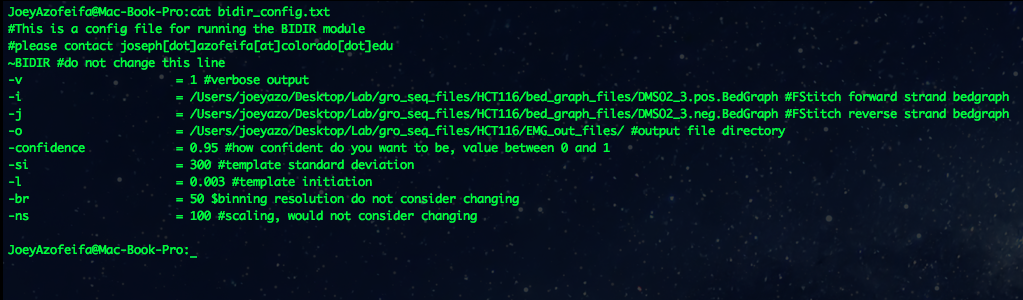
\includegraphics[width=\linewidth]{/Users/joeyazo/Desktop/Lab/EMG/tutorial/latex/images/config_example}
\\
\\
The first line is a just a header. The second line with the tilda sign, signifies the module that this config is specific for. This line should not be changed. The rest of the lines list the parameter and their associate value. These parameters can be changed by simply replaced the number or the file path in between the equals sign and the pound sign. 
\\
\\
Indeed, you can also overwrite any parameters in the config file by supplying them in the command line. With the above examble, $-l$ is set to 0.003 to overwrite this at run time you can do, 
\\
\\
bash-terminal\$ ./EMGU bidir\_config.txt $-l$ 0.1
\\
\\
and 0.1 will be the parameter to the program not 0.003.

\section{Bidirectional Detector }
\subsection{Method Description}

The simplest way to identify regions of the genome that have bidirectional transcription is to compare model fits between an elongation component and a bidirectional component and simply perform a template matching algorithm to identify good hits. Thus we slide the center of loading or $\mu$
in $f(z,s)$ and compare the likelihoods via Bayesian Information Criteria (BIC) to a bidirectional fit verse noise or elongation fit. Thusly we compute this score for every position in the genome:

\begin{displaymath}
\begin{split}
ll_f 		= \sum_{i=j}^{k} \log{f(z_i, s_i)}&; ll_g = \sum_{i=j}^{k} \log{g(z_i, s_i)}\\
BIC_f 	= -2\cdot ll_f  + 5\cdot\log{N}&;BIC_g 	= -2\cdot ll_g +2\cdot\log{N}\\
SCORE 	&= BIC_g/BIC_f \\
\end{split}\numberthis \label{eqn_4}
\end{displaymath}
If this score is above one, than the likelihood of this window being in the bidirectional component is greater than that of the uniform component. To compute this score, we must fix the variance and initiating parameter of the EMG component. We let users play with this number but I have found that variance around ($\sigma$) 300 and initiating parameter ($\lambda$) at 0.003 to be the best as this is the global average parameter estimates across single isoform genes in the HCT116 DMSO GRO-seq (however this number may change from dataset to datasets...users are encouraged to figure out this number for themselves by running below modules on single isoform genes). The window is simply one standard deviation to the right and to the left of some genome position and thus is a function of the user provided $\sigma$ and $\lambda$ options. Lastly the user can provide a confidence threshold, anything above 0.95 would be considered highly significant, decreasing this parameter will lead to more bidirectional calls. 

\subsection{Parameter Description}

\begin{center}
\begin{tabular}{ |c|c|c| } 
 \hline
 Flag & Type & Description \\ 
 \hline
 \hline
 -i & string;/path/to/file/ & forward strand bed graph file \\ 
 \hline
 -j & string;/path/to/file/ & reverse strand bed graph file \\ 
 \hline
 -o & string;/path/to/directory/ & output directory (bidirectional\_hits.bed created) \\ 
 \hline
 -confidence & number(float/double) & score confidence \\ 
 \hline
 -si & number(float/double) & EMG template $\sigma$ \\ 
 \hline
 -l & number(float/double) & EMG template $\lambda$ \\ 
 \hline
 -br & number(float/double) & binning resolution*** \\ 
 \hline
-ns & number(float/double) & normalizing scale*** \\ 
 \hline
 \hline
&&***Would not consider changing\\ 
 \hline
\end{tabular}
\end{center}


\section{Formatting Data}
\subsection{Method Description}
\subsection{Parameter Description}
\begin{center}
\begin{tabular}{ |c|c|c| } 
 \hline
 Flag & Type & Description \\ 
 \hline
 \hline
 -i & string;/path/to/file/ & bed file of intervals \\ 
 \hline
 -j & string;/path/to/file/ & forward strand bed graph file \\ 
 \hline
 -k & string;/path/to/file/ & reverse strand bed graph file \\ 
 \hline
 -o & string;/path/to/directory/ & output directory (EMGU\_formatted\_file.tsv created) \\ 
 \hline
 -pad & number, integer & additional data inserted to interval \\ 
 \hline
\end{tabular}
\end{center}


\section{Estimating Parameters}
\subsection{Method Description}
\subsection{Parameter Description}
\begin{center}
\begin{tabular}{ |c|c|c| } 
 \hline
 Flag & Type & Description \\ 
 \hline
 \hline
 -i & string;/path/to/file/ & EMGU\_formatted\_file.tsv, (output from FORMAT module) \\ 
 \hline
 -o & string;/path/to/file/ & output directory (model\_fits.tsv) will be created \\ 
 \hline
 -np & number(integer) & number of CPU cores \\ 
 \hline
 -chr & string; chr\# or all & run on a specific chromosome or on all \\ 
 \hline
 -br & number(float/double) & binning resolution*** \\ 
 \hline
-ns & number(float/double) & normalizing scale*** \\ 
 \hline
 -minK & number(integer) & do not consider models with less than this many component \\ 
 \hline
 -maxK & number(integer) & do not consider models with more than this many component \\ 
 \hline
 -rounds & number(integer) & number of random EM initializations \\ 
 \hline
 -ct & number(float/double) & EM convergence threshold difference \\ 
 \hline
 -mi & number(integer) & Number of EM iterations before it is aborted \\ 
 \hline
 -mi & number(integer) & Number of EM iterations before it is aborted \\ 
 \hline
 -max\_noise & number(float/double) & weight of the random/uniform noise component*** \\ 
 \hline
 -ALPHA\_0 & number(float/double) & hyper parameter for $\sigma$,$NIG$(ALPHA\_0, BETA\_0)*** \\ 
 \hline
 -BETA\_0 & number(float/double) & hyper parameter for $\sigma$,$NIG$(ALPHA\_0, BETA\_0)*** \\ 
 \hline
 -ALPHA\_1 & number(float/double) & hyper parameter for $\lambda$,$\Gamma$(ALPHA\_1, BETA\_1)*** \\ 
 \hline
 -BETA\_1 & number(float/double) & hyper parameter for $\lambda$,$\Gamma$(ALPHA\_1, BETA\_1)*** \\ 
 \hline
 -ALPHA\_2 & number(float/double) & beta hyper parameter for strand bias*** \\ 
 \hline
 -ALPHA\_3 & number(float/double) & dirchlet hyper parameter for component weights*** \\ 
 \hline
 \hline
&&***Would not consider changing\\ 
 \hline


\end{tabular}
\end{center}

\section{Model Selection}
\subsection{Method Description}
\subsection{Parameter Description}
 \begin{center}
\begin{tabular}{ |c|c|c| } 
 \hline
 Flag & Type & Description \\ 
 \hline
 \hline
 -i & string;/path/to/directoy/ &directory of model\_fit.tsv files, (output of MODEL module) \\ 
 \hline
 -o & string;/path/to/file/ & output directory (model\_fits.txt and/or model\_fits.bed created) \\ 
 \hline
 -penailty & number;(float/double) & BIC penalty*** \\ 
 \hline
 -to\_igv & 0/1 & output a file to view in IGV/UCSC browser viewing \\ 
 \hline
 -to\_EMG & 0/1 & output a file in format as from MODEL module \\ 
 \hline
\end{tabular}
\end{center}

\section{File Type Appendix} 
 
\end{document}